\section{Introduction}

Joining two datasets is a key step in preparing the data for subsequent operations such as performing business analytics, building predictive models etc.  Data management systems have largely focussed solely on equi-joins, which is based on exact equality of strings or numeric values.  However, in many circumstances, exact equality is inadequate because the same entity may in many cases be expressed with slight variations of the same name, as shown in Figure~\ref{table-example} (e.g., \textit{Douglas Adams} and \textit{Douglas Noel Adams}).  Although Figure~\ref{table-example} illustrates the problem for people's names, the same problem occurs for other entity types, such as company names, addresses, states in countries, and countries.

One common technique to automating joins of the sort described in Figure \ref{table-example} is string matching.  String matching approaches use variants of string similarity measures such as edit-distance, Jaro-Winkler and TF-IDF (e.g., \cite{Cohen2003}) to perform matching.  Typically to scale the problem to a large number of rows in each table, a filtering or blocking strategy is used to reduce the number of pairs to be considered for string matching.  For instance, prefix, string length, or suffix based filtering are often applied to the strings in the two tables to identify potentially joinable pairs that need to be matched.  For the examples shown in Figure~\ref{table-example}, the prefix filtering step will ensure that \textit{Douglas Adams} will be compared only with \textit{Douglas Noel Adams} and \textit{Doug C. Engelbart} to determine their string similarity, assuming the prefix used for filtering is \textit{Doug}.  

More recently, data driven approaches have emerged as a powerful alternative to string matching techniques for the join problem described in Figure~\ref{table-example}.  Data driven approaches mine patterns in the data to determine the `rules' for joining a given entity type.  One example of such an approach is illustrated in \cite{He:2015:SJS:2824032.2824036}, which determines which cell values should be joined based on whether those cell values co-occur on the same row across disparate tables in a very large corpus of data.  Such a system can perform `semantic joins' such as mapping country names to country codes in new unseen tables.  Another example of a data driven approach is work by \cite{auto-join-joining-tables-leveraging-transformations} that uses program synthesis techniques to learn the right set of transformations needed to perform the entity matching operation, based on a numerous examples.  Unlike string matching algorithms, which apply the same generic operator to a cell value regardless of entity type, the approach outlined in \cite{auto-join-joining-tables-leveraging-transformations} can learn different programs to transform cell values for different entity types. 

In this paper, we propose a novel data driven approach to the problem of joining semantically different representations of data.  Our approach relies on building supervised deep learning models to automatically learn the correct set of transformations needed to compute the equality of two cell values.  Because a deep learning model can pick up the appropriate features of what should be used for matching from correlations in the data, it should in theory be able to generalize better across join problems than the data driven approaches outlined in \cite{He:2015:SJS:2824032.2824036}.   Conceptually, our approach is similar in spirit to the approach described in \cite{auto-join-joining-tables-leveraging-transformations}, but we use deep neural networks to learn the right function for the join operation instead of synthesizing different programs for different entity types.  The advantage of building such a function over the approach described in \cite{auto-join-joining-tables-leveraging-transformations} is that we can use this function in novel ways to completely eliminate the filtering that is typically needed to identify the set of potentially joinable rows, as we describe below.  

Our specific solution to the join problem involves building a deep neural network that learns to produce a small distance estimate for elements of a name pair that represent the same entity (e.g., \textit{Douglas Adams}-\textit{Douglas Noel Adams} should produce a distance estimate $d$ that is closest to 0), and a much larger distance estimate for elements of the name pair that do not represent the same entity (e.g., \textit{Douglas Adams}-\textit{John Adams} should produce a distance estimate $d$ that is greater than some margin $m$).  The function learnt by such a network (often called a `siamese network') is conceptually one that maps input vectors for the same entity closer together in vector space, while mapping input vectors for a different entity to a distance that is at least \textit{m} distance away from the vectors for the same entity, as shown in Figure \ref{fig-1}.  This sort of function can be used to determine join equality on a subset of string pairs that are considered joinable using some sort of filtering step, as is often done in approaches to the semantic join type problem (e.g. \cite{auto-join-joining-tables-leveraging-transformations}).  

However, our observation is that one can actually exploit what the siamese network produces to eliminate this filtering step altogether.  Specifically, the last hidden layer of the siamese network is effectively a `vector embedding' for the same versus different estimate.  That is, the last layer is a vector in a lower dimensional space that contains the critical features needed for computing the distance estimate.  We can in fact take these vector embeddings for all vectors in the two tables to be joined, and use approximate nearest neighbors algorithms to find the nearest neighbors.  Ideally, the nearest neighbor that has a distance lower the margin $m$ should be the correct match.  Because approximate nearest neighbor algorithms have been applied successfully to millions of items, this approach should scale just as well as filtering/join algorithms, but have the added advantage that the filtering step is also data driven, and hence can adapt to different entity types very effectively.

\begin{figure}
\centering
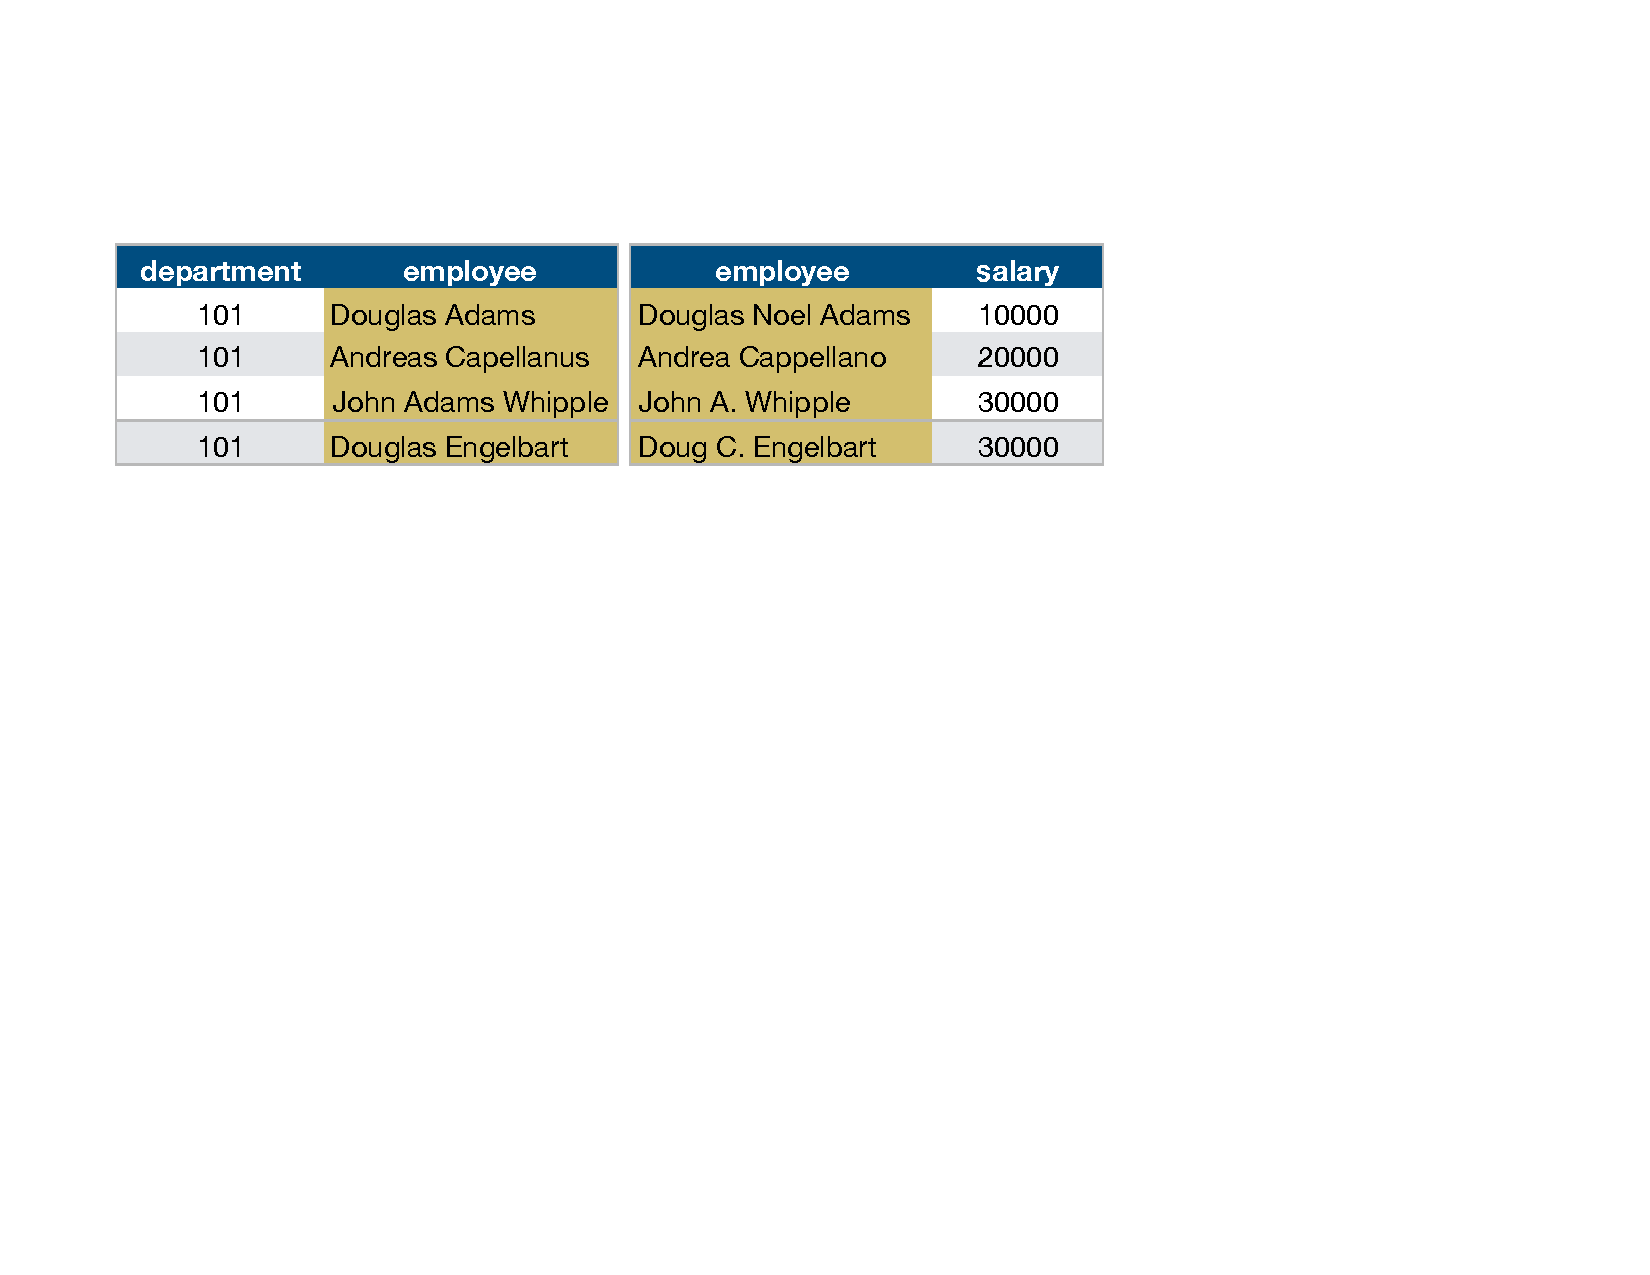
\includegraphics[width=1\linewidth]{fig1}
\label{table-example}
\caption{Example of a join problem}
\end{figure}


\begin{figure}
\centering
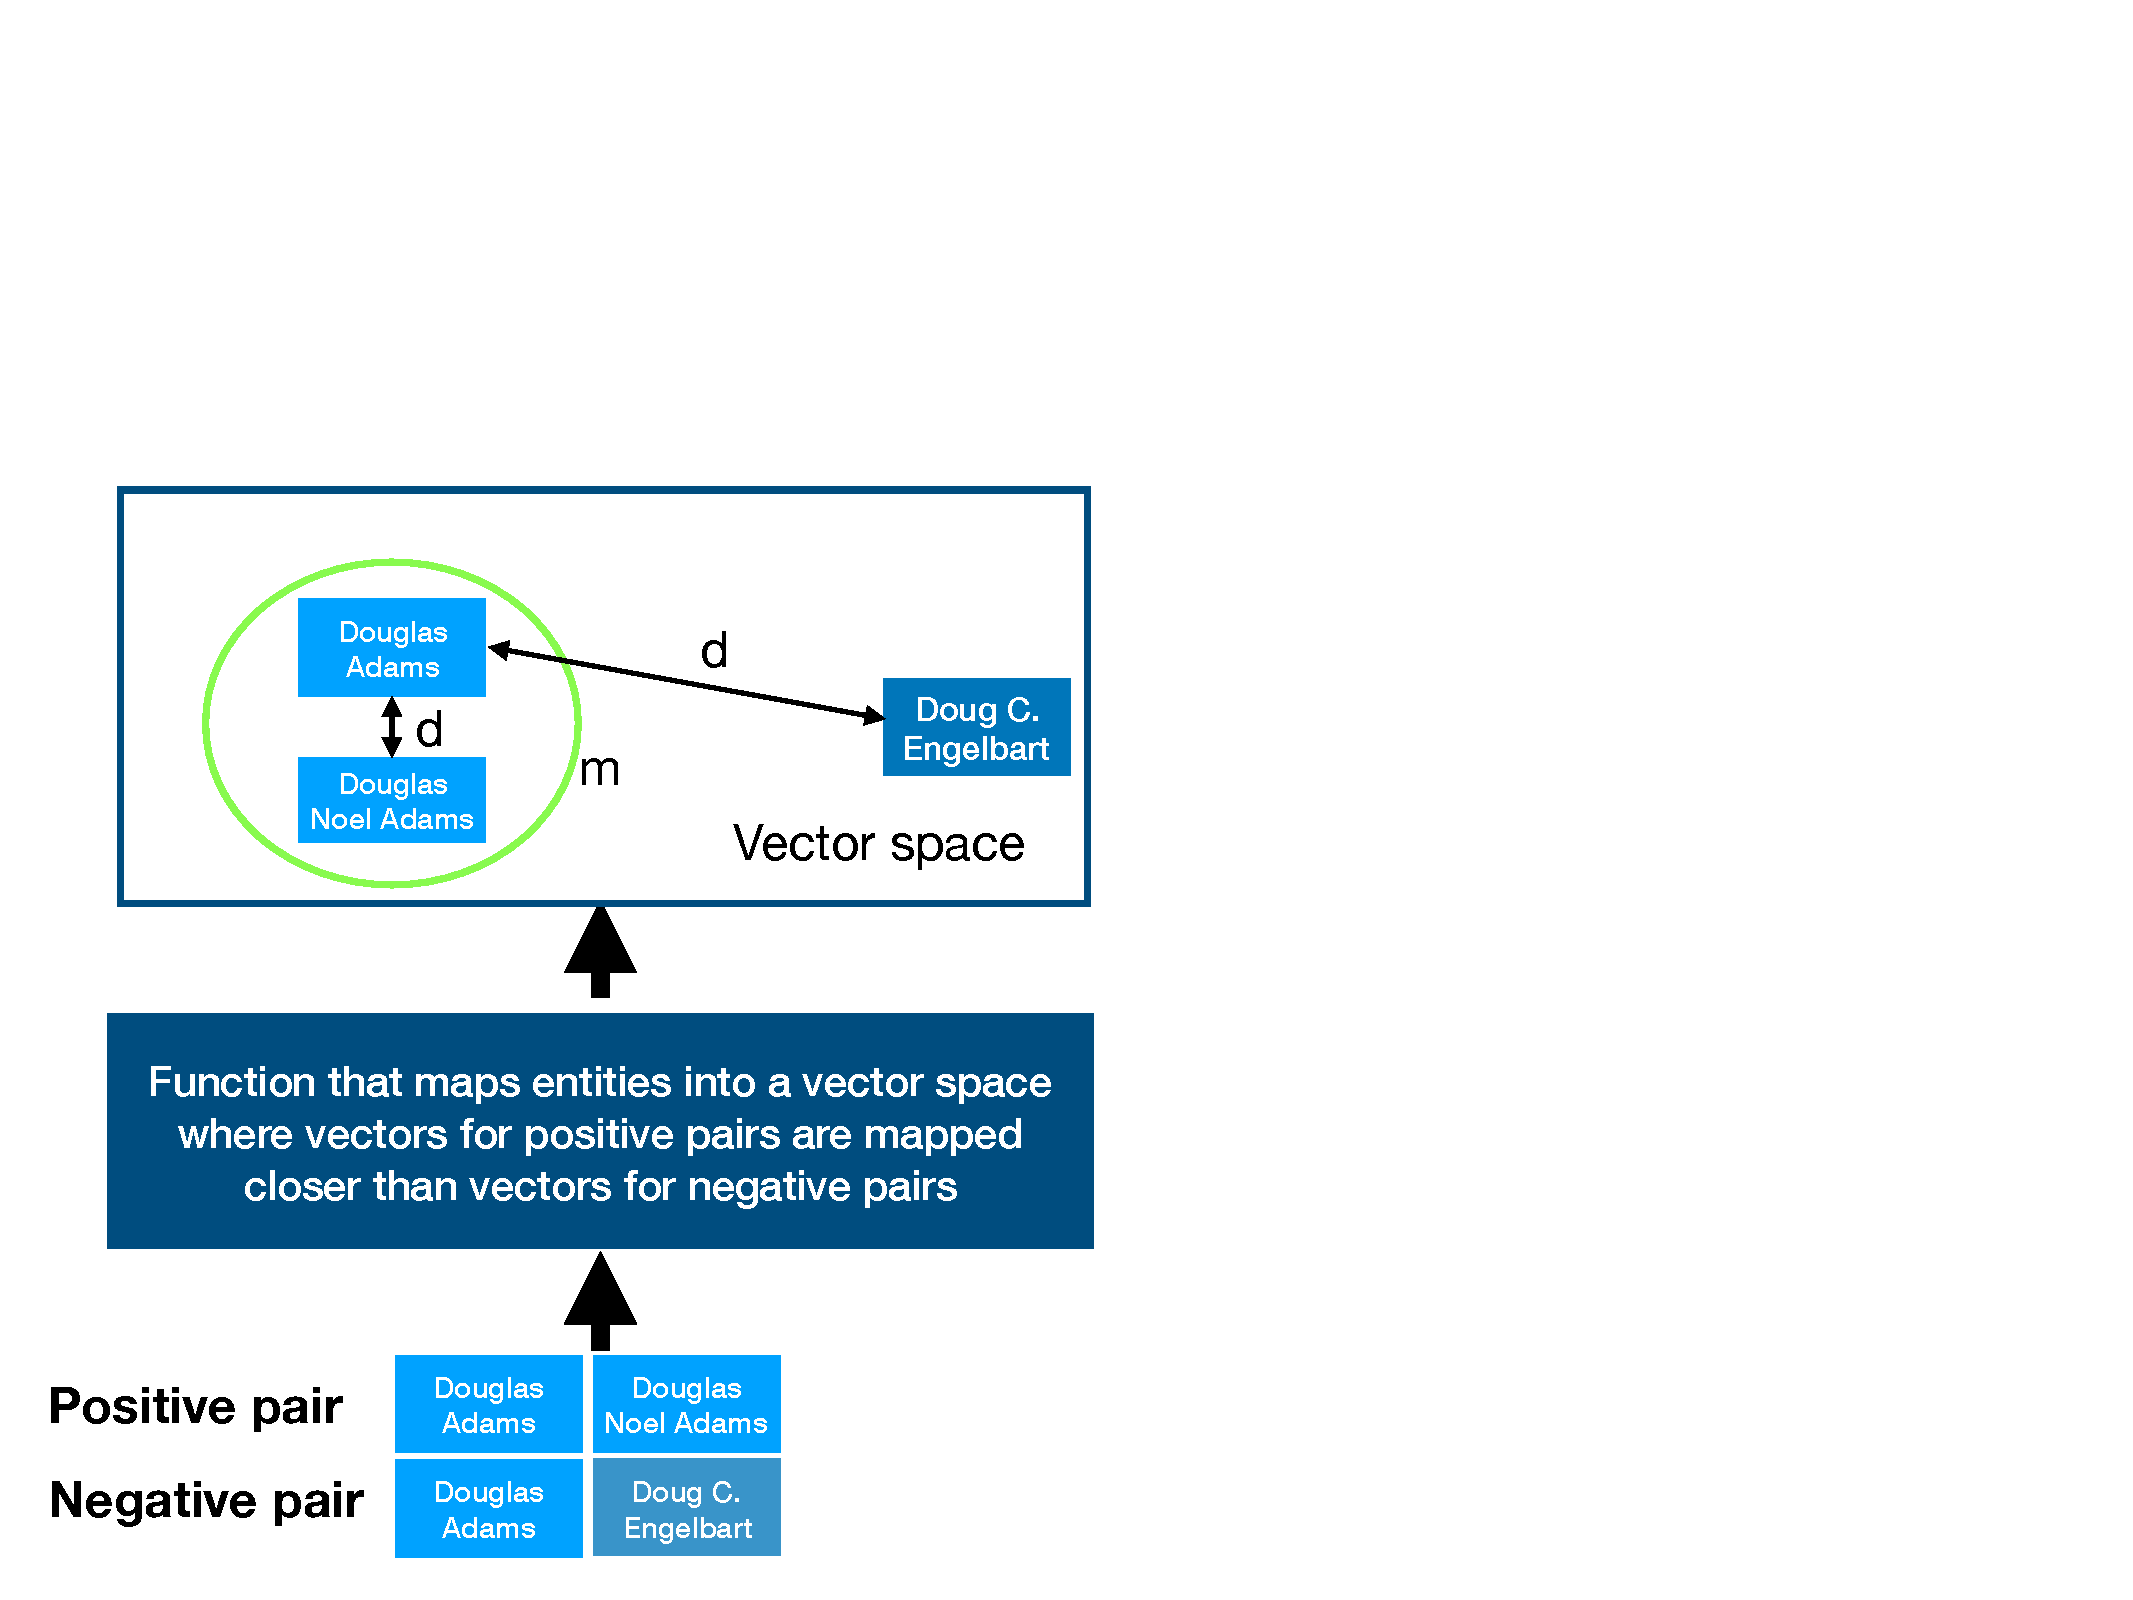
\includegraphics[width=1\linewidth]{fig2}
\label{fig-1}
\caption{Conceptual overview of neural network approach to matching}
\end{figure}

Our key contributions to the join problem are as follows:
\begin{itemize}
\item We demonstrate that we can use a triplet loss network to learn a distance function that successfully discriminates same pairs from different pairs with an accuracy of 97\%.  Our results suggest that deep learning models can be used successfully as another mechanism for data driven joins, assuming some sort of filtering approach has been applied to the data.
\item We try to extend this further; to see if the output of the function can in fact be used in an approximate nearest neighbor algorithm to identify neighbors to match with, without any filtering. 
\end{itemize}

